\subsection{Sprzęt}

Stworzenie wystarczająco jak na potrzeby niniejszego projektu rozbudowanej
infrastruktury niesie ze sobą konieczność wyboru sprzętu, na którym poszczególne
elementy składowe będą uruchomione. Ponieważ część kliencka (interfejs)
uruchamiana jest na komputerach użytkowników (klientów i pracowników) należy
podjąć decyzję co do wyboru sprzętu, na którym znajdowałby się serwer
aplikacyjny oraz serwery bazodanowe.

Jako serwer aplikacyjny zdecydowano się wykorzystać \emph{Dell PowerEdge R710}.
Charakteryzuje się on wysoką wydajnością przy jednoczesnym stosunkowo małym
poborze prądu i wysokiej jakości wykonania.

\begin{figure}[h!]
    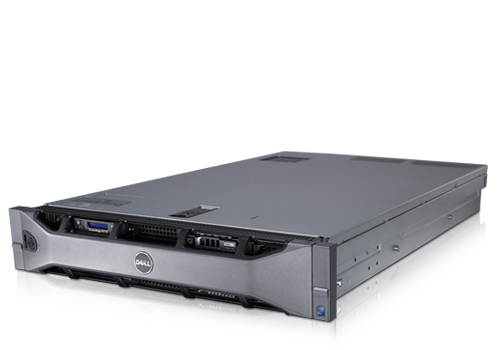
\includegraphics[width=\textwidth,
    height=0.2\textheight]{graphics/SerwerAplikacyjny.jpg}
  \caption{Wykorzystany moduł aplikacyjny}
\end{figure}

Specyfikacja techniczna serwera aplikacyjnego:

\begin{enumerate}
  \item Chipset - Intel 5520
  \item Pamięć - Do 192 GB2 (18 gniazd DIMM): 1 GB/2 GB/4 GB/8 GB/16 GB DDR3 800
  MHz, 1066 MHz lub 1333 MHz
  \item Maksymalna pojemność wewnętrznej pamięci masowej - 18 TB
  \item Gniazda - 2 PCIe x8 + 2 PCIe x4 G2 lub 1 x16 + 2 x4 G2
  \item Zasilanie - Dwa zasilacze awaryjne typu hot-plug 570 W o wysokiej sprawności ALBO dwa zasilacze awaryjne typu hot-plug 870 W o wysokiej mocy
  
\end{enumerate}


Specyfikacja bazodanowa (Oracle 11.2) wymaga także wydajnego i szybkiego
serwera, dzięki któremu dane będą zarówno pobierane jak i wstawiane w sposób
optymalny. Dlatego też zdecydowano się na serwer \emph{Dell PowerEdge R720}:

\begin{figure}[h!]
    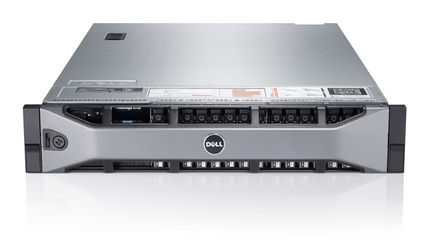
\includegraphics[width=\textwidth,
    height=0.2\textheight]{graphics/SerwerBazodanowy.jpg}
  \caption{Wykorzystany moduł bazy danych}
\end{figure}


Specyfikaczna techniczna serwera bazy danych:

\begin{enumerate}
  \item Liczba gniazd procesorów - 2
  \item Chipset - Intel C600
  \item Pamięć - Do 768 GB (24 gniazda DIMM) w modułach DDR3 2 GB/4 GB/8 GB/16
  GB/32 GB o częstotliwości do 1866 MT/
  \item Maksymalna pojemność wewnętrznej - 32 TB
  \item Gniazda - 7 gniazd PCIe:
	Jedno gniazdo x16 pełnej długości i wysokości 
	Trzy gniazda x8 pełnej długości i wysokości
	Trzy gniazda x8 o połowie długości i wysokości
  \item Zasilanie - Nadmiarowy zasilacz hot-plug o sprawności klasy Titanium i mocy 750 W
	Nadmiarowe zasilacze hot-plug o sprawności klasy Platinum i mocy 495 W, 750 W
	lub 1100 W Zasilacze z funkcją automatycznego wykrywania zakresu
\end{enumerate}
